\subsection*{Cornelia Castle}
A map of the ground floor is shown below, where relevant locations are numbered according to their paragraphs.
The stairs in the center lead to the throne room, while the entrance in the back leads to the palace garden, which is currently closed off.
The palace is filled with armed guards at all times.
\begin{center} 
	\tcbox[left=0pt,top=0pt,right=0pt,bottom=0pt, boxsep=0pt, colframe=accent, sharp corners]{
		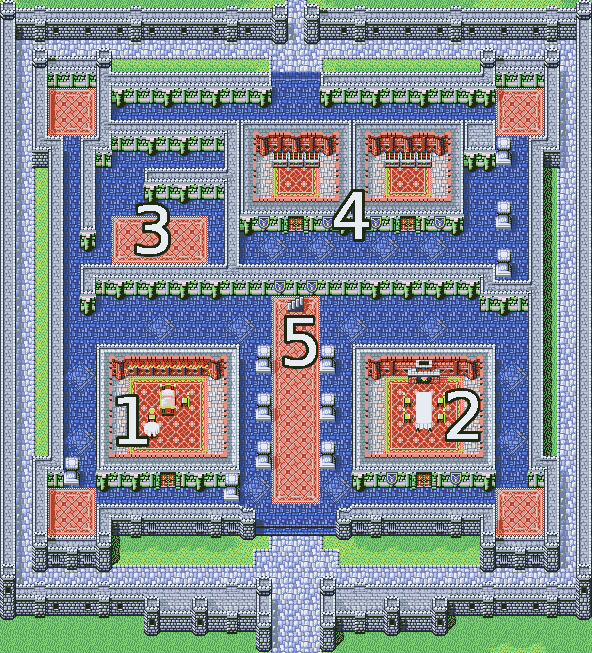
\includegraphics[width=0.98\columnwidth]{./art/maps/castle.png} 
	}
\end{center}
\subsubsection*{1. Queen's Room}
"Please... please bring my daughter... my Sarah... back to me safely."
\indent -- Queen Jayne \\\\
Queen Jayne is a middle-aged women with turquoise hair and blue eyes, wearing a well-made long red dress and a golden tiara.
She has been depressed since her daughter's kidnapping and only talks to the party after they have won the king's trust.
Once she talks, she tells the party about the night of the kidnapping, which she has witnessed personally.
On that night, she woke up and encountered Garland who was escaping with the unconscious princess in his arms.
Garland told her to hand over control Cornelia if she wants to see her daughter alive again.
Then he disappeared with Sarah through the back entrance of the palace.
The Queen is traumatized by this event and she blames herself for not preventing the kidnapping.

\subsubsection*{2. Sisters's Room}
"My s-s-sister... W-where's my s-sister?"
\indent -- Alison\\\\
This room is inhabited by Sarah's sister Alison who is an emotional teenager, that resembles her mother.
The guards at her door tell the party that she has locked herself in and won't open the door.
If the party can convince her, e.g. by assuring that they will save Sarah, she opens the door to talk.
Alison knows her sister well, as she looks up to her very much.
She tells the party about Sarah's passion for music and that her precious lute has disappeared with her.
If the party manages to calm Alison down, they have a better chance at convincing the king, who is worried about her. 

\subsubsection*{3. Captain}
"Garland was once the greatest knight in the kingdom. But power corrupted him, and he turned away from his own true nature."
\indent -- Ian \\\\
The captain of the guard is a young man with long blond hair named Ian, he is wearing a decorated heavy armor and a longsword on his back.
He is reluctant to talk the adventurers and they immediately notice that he is missing his left arm. 
If the party has convinced the king, the captain is willing to talk to them about the mission to rescue Sarah, which he led.
Right after Sarah disappeared, him his men followed Garland and confronted him at the Big Bridge, north of Cornelia.
However, Garland bested all of them in ensuing battle and the captain was the only one to survive, albeit without his arm.
He is ashamed of his failure and seems deeply disturbed and scared of Garland's power.

\subsubsection*{4. Treasure Room}
The treasury consists of two rooms, the one to the left contains the palace's gold while the right one contains expensive items and equipment.
Both doors are guarded by two well armed men in heavy armor.
If the party has obtained a letter from the king, they are given the following items by guards: 
A large Tent that fits the entire party as well as a Potion and 200 Gil per party member.

\subsubsection*{5. Throne Room}
The door is guarded by two royal guards with glaives and heavy decorated armor.
Inside the throne room, the king sits on his throne and beside him stands the chancellor.
The king is a middle-aged man with light blue eyes and brown hair with a long brown beard, he is wearing a golden crown and long red robes.
The chancellor is slightly younger with dark hair, also wearing noble clothing.
The king is happy to see the adventurers, as he is desperate to find his daughter, but the chancellor is very skeptical.
In the following conversation, the party can try to convince the king that they can rescue Sarah, but the chancellor convinces him that they have to prove their trustworthiness first.
The king then laments that he has been neglecting his people while trying to rescue his daughter.
He asks the party to help the people of Cornelia to prove that they are capable of saving Sarah, in return he promises to provide them with supplies for the journey.
If the party asks for further details on the kidnapping, they do not reveal anything until the party has won their trust.

\subsubsection*{Convincing the King}
"Garland is no longer the man I once knew... I beg of you. Please return my daughter to me quickly!"

\indent -- King of Cornelia \\\\
To convince the king, the party has to fulfil a number of tasks that help the people of Cornelia, which ones and how many exactly depends on you as the GM.
Below is a list of tasks that may convince the king if taken care of:
\begin{itemize}[leftmargin=*]
	\item Help the smith to receive his shipments.
	\item Resolve the dispute between the two mages.
	\item Defend the port against an ambush by pirates.
	\item Help the chapel regain its members.
\end{itemize}
After the party wins the king's trust, he reveals further details on the kidnapping:
Sarah was kidnapped by a former knight of Cornelia named Garland, the most powerful swordsman in the kingdom.
Garland used to be close to the king, but power has corrupted him and he demanded to become his successor. 
When the king denied him, Garland abducted his daughter Sarah as ransom for control over Cornelia.
Many other knights have tried to save her since and even though none succeeded, they found out that Garland keeps Sarah in the Chaos Shrine, north of Cornelia past the Big Bridge.
The king keeps his promise and writes a letter to confirm that they were officially given the task of rescuing the princess.
This letter allows the party to retrieve supplies from the treasury and other members of the palace are more willing to talk to them.
After successfully convincing the king, the party is rewarded with a \textbf{Level Up}!
\vspace{1.2cm}